\documentclass{standalone}
\usepackage{tikz}
\usetikzlibrary{patterns, positioning}


\begin{document}
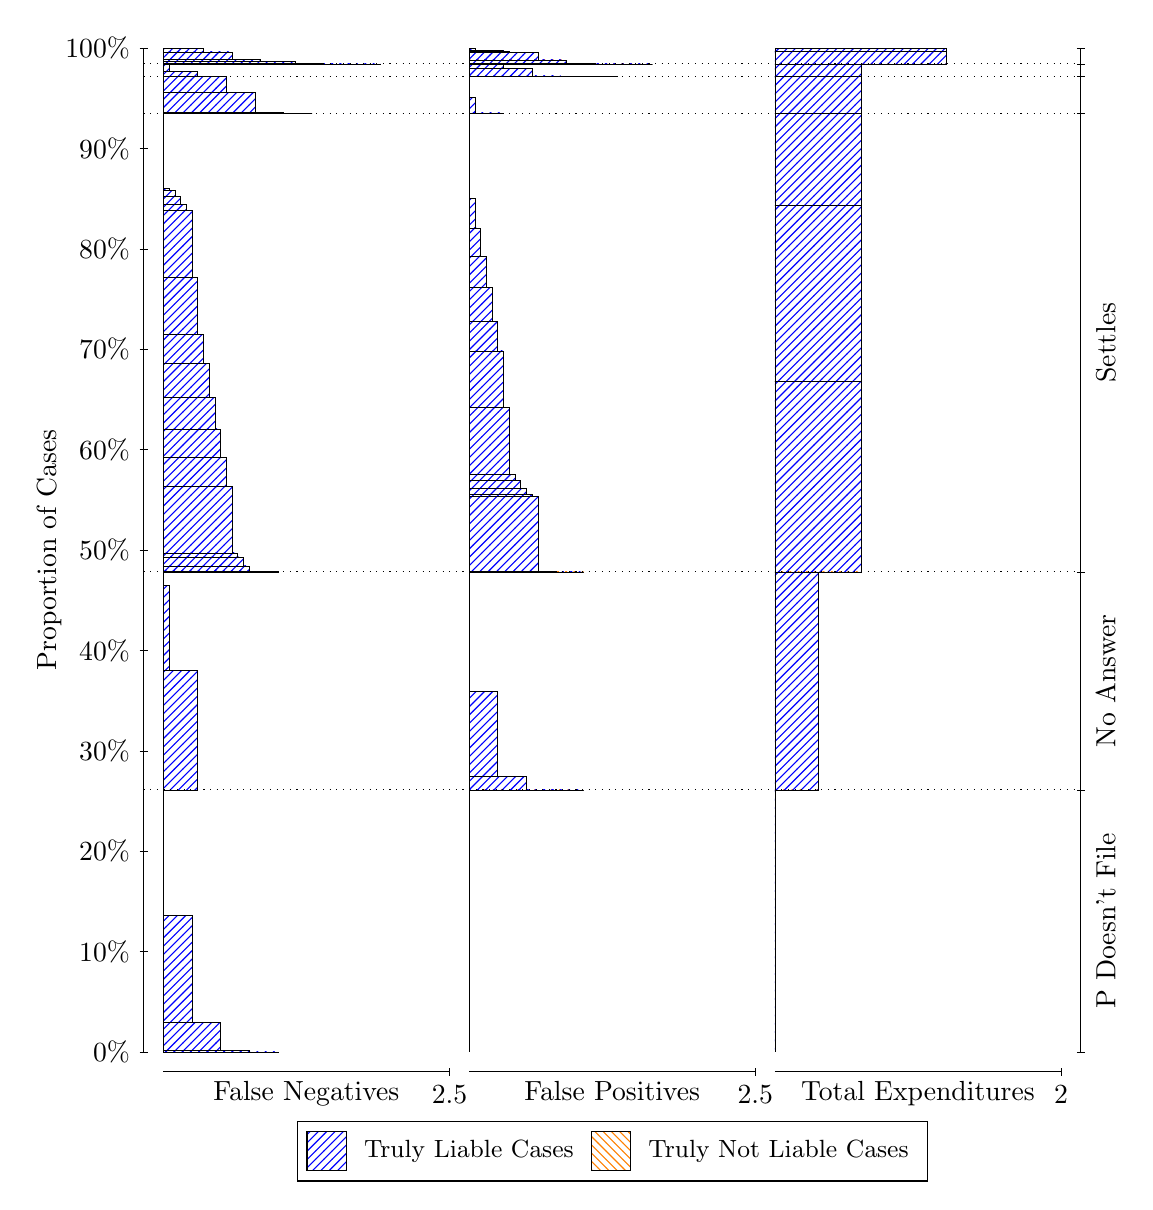
\begin{tikzpicture}
\draw[black, very thin] (1.5,1.75) -- (1.5,14.5);
\node[rotate=90, text=black, anchor=center] at (0.3, 8.125) {Proportion of Cases};
\draw[black, very thin] (1.45,1.75) -- (1.55,1.75);
\node[text=black, anchor=east] at (1.45, 1.75) {0\%};
\draw[black, very thin] (1.45,3.025) -- (1.55,3.025);
\node[text=black, anchor=east] at (1.45, 3.025) {10\%};
\draw[black, very thin] (1.45,4.3) -- (1.55,4.3);
\node[text=black, anchor=east] at (1.45, 4.3) {20\%};
\draw[black, very thin] (1.45,5.575) -- (1.55,5.575);
\node[text=black, anchor=east] at (1.45, 5.575) {30\%};
\draw[black, very thin] (1.45,6.85) -- (1.55,6.85);
\node[text=black, anchor=east] at (1.45, 6.85) {40\%};
\draw[black, very thin] (1.45,8.125) -- (1.55,8.125);
\node[text=black, anchor=east] at (1.45, 8.125) {50\%};
\draw[black, very thin] (1.45,9.4) -- (1.55,9.4);
\node[text=black, anchor=east] at (1.45, 9.4) {60\%};
\draw[black, very thin] (1.45,10.675) -- (1.55,10.675);
\node[text=black, anchor=east] at (1.45, 10.675) {70\%};
\draw[black, very thin] (1.45,11.95) -- (1.55,11.95);
\node[text=black, anchor=east] at (1.45, 11.95) {80\%};
\draw[black, very thin] (1.45,13.225) -- (1.55,13.225);
\node[text=black, anchor=east] at (1.45, 13.225) {90\%};
\draw[black, very thin] (1.45,14.5) -- (1.55,14.5);
\node[text=black, anchor=east] at (1.45, 14.5) {100\%};

\draw[black, very thin] (13.4,1.75) -- (13.4,14.5);
\draw[black, very thin] (13.35,1.75) -- (13.45,1.75);
\node[anchor=west] at (13.35, 1.75) {};
\draw[black, very thin] (13.35,5.0788) -- (13.45,5.0788);
\node[anchor=west] at (13.35, 5.0788) {};
\draw[black, very thin] (13.35,7.8475) -- (13.45,7.8475);
\node[anchor=west] at (13.35, 7.8475) {};
\draw[black, very thin] (13.35,13.674) -- (13.45,13.674);
\node[anchor=west] at (13.35, 13.674) {};
\draw[black, very thin] (13.35,14.138) -- (13.45,14.138);
\node[anchor=west] at (13.35, 14.138) {};
\draw[black, very thin] (13.35,14.299) -- (13.45,14.299);
\node[anchor=west] at (13.35, 14.299) {};
\draw[black, very thin] (13.35,14.5) -- (13.45,14.5);
\node[anchor=west] at (13.35, 14.5) {};

\draw[black, very thin, pattern color=blue, pattern=north east lines] (1.75,1.75) rectangle (3.2033,1.7502);
\draw[black, very thin, pattern color=blue, pattern=north east lines] (1.75,1.7502) rectangle (2.84,1.7747);
\draw[black, very thin, pattern color=blue, pattern=north east lines] (1.75,1.7747) rectangle (2.4767,2.1245);
\draw[black, very thin, pattern color=blue, pattern=north east lines] (1.75,2.1245) rectangle (2.1133,3.4874);
\draw[black, very thin, pattern color=orange, pattern=north west lines] (1.75,3.4874) rectangle (1.75,3.4874);
\draw[black, very thin, pattern color=blue, pattern=north east lines] (1.75,3.4874) rectangle (1.75,5.0788);
\draw[black, very thin, pattern color=blue, pattern=north east lines] (1.75,5.0788) rectangle (2.186,6.5988);
\draw[black, very thin, pattern color=blue, pattern=north east lines] (1.75,6.5988) rectangle (1.8227,7.678);
\draw[black, very thin, pattern color=orange, pattern=north west lines] (1.75,7.678) rectangle (1.75,7.678);
\draw[black, very thin, pattern color=blue, pattern=north east lines] (1.75,7.678) rectangle (1.75,7.8475);
\draw[black, very thin, pattern color=blue, pattern=north east lines] (1.75,7.8475) rectangle (3.2033,7.8494);
\draw[black, very thin, pattern color=blue, pattern=north east lines] (1.75,7.8494) rectangle (3.058,7.8495);
\draw[black, very thin, pattern color=blue, pattern=north east lines] (1.75,7.8495) rectangle (2.9127,7.8601);
\draw[black, very thin, pattern color=blue, pattern=north east lines] (1.75,7.8601) rectangle (2.84,7.9245);
\draw[black, very thin, pattern color=blue, pattern=north east lines] (1.75,7.9245) rectangle (2.7673,8.0376);
\draw[black, very thin, pattern color=blue, pattern=north east lines] (1.75,8.0376) rectangle (2.6947,8.0887);
\draw[black, very thin, pattern color=blue, pattern=north east lines] (1.75,8.0887) rectangle (2.622,8.9298);
\draw[black, very thin, pattern color=blue, pattern=north east lines] (1.75,8.9298) rectangle (2.5493,9.3058);
\draw[black, very thin, pattern color=blue, pattern=north east lines] (1.75,9.3058) rectangle (2.4767,9.6645);
\draw[black, very thin, pattern color=blue, pattern=north east lines] (1.75,9.6645) rectangle (2.404,10.06);
\draw[black, very thin, pattern color=blue, pattern=north east lines] (1.75,10.06) rectangle (2.3313,10.495);
\draw[black, very thin, pattern color=blue, pattern=north east lines] (1.75,10.495) rectangle (2.2587,10.867);
\draw[black, very thin, pattern color=blue, pattern=north east lines] (1.75,10.867) rectangle (2.186,11.586);
\draw[black, very thin, pattern color=blue, pattern=north east lines] (1.75,11.586) rectangle (2.1133,12.44);
\draw[black, very thin, pattern color=blue, pattern=north east lines] (1.75,12.44) rectangle (2.0407,12.515);
\draw[black, very thin, pattern color=blue, pattern=north east lines] (1.75,12.515) rectangle (1.968,12.617);
\draw[black, very thin, pattern color=blue, pattern=north east lines] (1.75,12.617) rectangle (1.8953,12.688);
\draw[black, very thin, pattern color=blue, pattern=north east lines] (1.75,12.688) rectangle (1.8227,12.715);
\draw[black, very thin, pattern color=orange, pattern=north west lines] (1.75,12.715) rectangle (1.75,12.715);
\draw[black, very thin, pattern color=blue, pattern=north east lines] (1.75,12.715) rectangle (1.75,13.674);
\draw[black, very thin, pattern color=blue, pattern=north east lines] (1.75,13.674) rectangle (3.6393,13.674);
\draw[black, very thin, pattern color=blue, pattern=north east lines] (1.75,13.674) rectangle (3.276,13.679);
\draw[black, very thin, pattern color=blue, pattern=north east lines] (1.75,13.679) rectangle (2.9127,13.939);
\draw[black, very thin, pattern color=blue, pattern=north east lines] (1.75,13.939) rectangle (2.5493,14.136);
\draw[black, very thin, pattern color=blue, pattern=north east lines] (1.75,14.136) rectangle (2.186,14.138);
\draw[black, very thin, pattern color=orange, pattern=north west lines] (1.75,14.138) rectangle (1.75,14.138);
\draw[black, very thin, pattern color=blue, pattern=north east lines] (1.75,14.138) rectangle (2.186,14.199);
\draw[black, very thin, pattern color=blue, pattern=north east lines] (1.75,14.199) rectangle (1.8227,14.292);
\draw[black, very thin, pattern color=orange, pattern=north west lines] (1.75,14.292) rectangle (1.75,14.292);
\draw[black, very thin, pattern color=blue, pattern=north east lines] (1.75,14.292) rectangle (1.75,14.299);
\draw[black, very thin, pattern color=blue, pattern=north east lines] (1.75,14.299) rectangle (4.5113,14.299);
\draw[black, very thin, pattern color=blue, pattern=north east lines] (1.75,14.299) rectangle (4.148,14.299);
\draw[black, very thin, pattern color=blue, pattern=north east lines] (1.75,14.299) rectangle (3.7847,14.303);
\draw[black, very thin, pattern color=blue, pattern=north east lines] (1.75,14.303) rectangle (3.712,14.303);
\draw[black, very thin, pattern color=blue, pattern=north east lines] (1.75,14.303) rectangle (3.4213,14.328);
\draw[black, very thin, pattern color=blue, pattern=north east lines] (1.75,14.328) rectangle (3.3487,14.328);
\draw[black, very thin, pattern color=blue, pattern=north east lines] (1.75,14.328) rectangle (3.058,14.334);
\draw[black, very thin, pattern color=blue, pattern=north east lines] (1.75,14.334) rectangle (2.9853,14.357);
\draw[black, very thin, pattern color=blue, pattern=north east lines] (1.75,14.357) rectangle (2.6947,14.357);
\draw[black, very thin, pattern color=blue, pattern=north east lines] (1.75,14.357) rectangle (2.622,14.451);
\draw[black, very thin, pattern color=blue, pattern=north east lines] (1.75,14.451) rectangle (2.3313,14.451);
\draw[black, very thin, pattern color=blue, pattern=north east lines] (1.75,14.451) rectangle (2.2587,14.498);
\draw[black, very thin, pattern color=blue, pattern=north east lines] (1.75,14.498) rectangle (1.8953,14.5);
\draw[black, very thin, pattern color=orange, pattern=north west lines] (1.75,14.5) rectangle (1.75,14.5);
\draw[black, very thin, pattern color=blue, pattern=north east lines] (1.75,14.5) rectangle (1.75,14.5);
\draw[black, very thin, pattern color=orange, pattern=north west lines] (5.6333,1.75) rectangle (5.6333,1.75);
\draw[black, very thin, pattern color=blue, pattern=north east lines] (5.6333,1.75) rectangle (5.6333,5.0788);
\draw[black, very thin, pattern color=orange, pattern=north west lines] (5.6333,5.0788) rectangle (7.0867,5.0788);
\draw[black, very thin, pattern color=blue, pattern=north east lines] (5.6333,5.0788) rectangle (7.0867,5.0788);
\draw[black, very thin, pattern color=blue, pattern=north east lines] (5.6333,5.0788) rectangle (6.7233,5.0794);
\draw[black, very thin, pattern color=blue, pattern=north east lines] (5.6333,5.0794) rectangle (6.36,5.2483);
\draw[black, very thin, pattern color=blue, pattern=north east lines] (5.6333,5.2483) rectangle (5.9967,6.3275);
\draw[black, very thin, pattern color=blue, pattern=north east lines] (5.6333,6.3275) rectangle (5.6333,7.8475);
\draw[black, very thin, pattern color=orange, pattern=north west lines] (5.6333,7.8475) rectangle (7.0867,7.8475);
\draw[black, very thin, pattern color=blue, pattern=north east lines] (5.6333,7.8475) rectangle (7.0867,7.8475);
\draw[black, very thin, pattern color=orange, pattern=north west lines] (5.6333,7.8475) rectangle (6.9413,7.8475);
\draw[black, very thin, pattern color=blue, pattern=north east lines] (5.6333,7.8475) rectangle (6.9413,7.8475);
\draw[black, very thin, pattern color=orange, pattern=north west lines] (5.6333,7.8475) rectangle (6.796,7.8475);
\draw[black, very thin, pattern color=blue, pattern=north east lines] (5.6333,7.8475) rectangle (6.796,7.8475);
\draw[black, very thin, pattern color=blue, pattern=north east lines] (5.6333,7.8475) rectangle (6.7233,7.8491);
\draw[black, very thin, pattern color=orange, pattern=north west lines] (5.6333,7.8491) rectangle (6.6507,7.8491);
\draw[black, very thin, pattern color=blue, pattern=north east lines] (5.6333,7.8491) rectangle (6.6507,7.8501);
\draw[black, very thin, pattern color=blue, pattern=north east lines] (5.6333,7.8501) rectangle (6.578,7.8512);
\draw[black, very thin, pattern color=orange, pattern=north west lines] (5.6333,7.8512) rectangle (6.5053,7.8512);
\draw[black, very thin, pattern color=blue, pattern=north east lines] (5.6333,7.8512) rectangle (6.5053,8.8065);
\draw[black, very thin, pattern color=blue, pattern=north east lines] (5.6333,8.8065) rectangle (6.4327,8.8334);
\draw[black, very thin, pattern color=blue, pattern=north east lines] (5.6333,8.8334) rectangle (6.36,8.9042);
\draw[black, very thin, pattern color=blue, pattern=north east lines] (5.6333,8.9042) rectangle (6.2873,9.0064);
\draw[black, very thin, pattern color=blue, pattern=north east lines] (5.6333,9.0064) rectangle (6.2147,9.0807);
\draw[black, very thin, pattern color=blue, pattern=north east lines] (5.6333,9.0807) rectangle (6.142,9.9352);
\draw[black, very thin, pattern color=blue, pattern=north east lines] (5.6333,9.9352) rectangle (6.0693,10.654);
\draw[black, very thin, pattern color=blue, pattern=north east lines] (5.6333,10.654) rectangle (5.9967,11.026);
\draw[black, very thin, pattern color=blue, pattern=north east lines] (5.6333,11.026) rectangle (5.924,11.461);
\draw[black, very thin, pattern color=blue, pattern=north east lines] (5.6333,11.461) rectangle (5.8513,11.857);
\draw[black, very thin, pattern color=blue, pattern=north east lines] (5.6333,11.857) rectangle (5.7787,12.215);
\draw[black, very thin, pattern color=blue, pattern=north east lines] (5.6333,12.215) rectangle (5.706,12.591);
\draw[black, very thin, pattern color=blue, pattern=north east lines] (5.6333,12.591) rectangle (5.6333,13.674);
\draw[black, very thin, pattern color=orange, pattern=north west lines] (5.6333,13.674) rectangle (6.0693,13.674);
\draw[black, very thin, pattern color=blue, pattern=north east lines] (5.6333,13.674) rectangle (6.0693,13.676);
\draw[black, very thin, pattern color=blue, pattern=north east lines] (5.6333,13.676) rectangle (5.706,13.873);
\draw[black, very thin, pattern color=blue, pattern=north east lines] (5.6333,13.873) rectangle (5.6333,14.138);
\draw[black, very thin, pattern color=orange, pattern=north west lines] (5.6333,14.138) rectangle (7.5227,14.138);
\draw[black, very thin, pattern color=blue, pattern=north east lines] (5.6333,14.138) rectangle (7.5227,14.138);
\draw[black, very thin, pattern color=blue, pattern=north east lines] (5.6333,14.138) rectangle (7.1593,14.138);
\draw[black, very thin, pattern color=blue, pattern=north east lines] (5.6333,14.138) rectangle (6.796,14.145);
\draw[black, very thin, pattern color=blue, pattern=north east lines] (5.6333,14.145) rectangle (6.4327,14.238);
\draw[black, very thin, pattern color=blue, pattern=north east lines] (5.6333,14.238) rectangle (6.0693,14.299);
\draw[black, very thin, pattern color=orange, pattern=north west lines] (5.6333,14.299) rectangle (7.9587,14.299);
\draw[black, very thin, pattern color=blue, pattern=north east lines] (5.6333,14.299) rectangle (7.9587,14.299);
\draw[black, very thin, pattern color=orange, pattern=north west lines] (5.6333,14.299) rectangle (7.5953,14.299);
\draw[black, very thin, pattern color=blue, pattern=north east lines] (5.6333,14.299) rectangle (7.5953,14.299);
\draw[black, very thin, pattern color=orange, pattern=north west lines] (5.6333,14.299) rectangle (7.232,14.299);
\draw[black, very thin, pattern color=blue, pattern=north east lines] (5.6333,14.299) rectangle (7.232,14.301);
\draw[black, very thin, pattern color=blue, pattern=north east lines] (5.6333,14.301) rectangle (6.8687,14.348);
\draw[black, very thin, pattern color=orange, pattern=north west lines] (5.6333,14.348) rectangle (6.8687,14.348);
\draw[black, very thin, pattern color=blue, pattern=north east lines] (5.6333,14.348) rectangle (6.8687,14.348);
\draw[black, very thin, pattern color=orange, pattern=north west lines] (5.6333,14.348) rectangle (6.796,14.348);
\draw[black, very thin, pattern color=blue, pattern=north east lines] (5.6333,14.348) rectangle (6.796,14.348);
\draw[black, very thin, pattern color=blue, pattern=north east lines] (5.6333,14.348) rectangle (6.5053,14.441);
\draw[black, very thin, pattern color=blue, pattern=north east lines] (5.6333,14.441) rectangle (6.5053,14.442);
\draw[black, very thin, pattern color=orange, pattern=north west lines] (5.6333,14.442) rectangle (6.4327,14.442);
\draw[black, very thin, pattern color=blue, pattern=north east lines] (5.6333,14.442) rectangle (6.4327,14.442);
\draw[black, very thin, pattern color=blue, pattern=north east lines] (5.6333,14.442) rectangle (6.142,14.456);
\draw[black, very thin, pattern color=blue, pattern=north east lines] (5.6333,14.456) rectangle (6.142,14.465);
\draw[black, very thin, pattern color=blue, pattern=north east lines] (5.6333,14.465) rectangle (6.0693,14.471);
\draw[black, very thin, pattern color=orange, pattern=north west lines] (5.6333,14.471) rectangle (6.0693,14.471);
\draw[black, very thin, pattern color=blue, pattern=north east lines] (5.6333,14.471) rectangle (6.0693,14.471);
\draw[black, very thin, pattern color=blue, pattern=north east lines] (5.6333,14.471) rectangle (5.7787,14.471);
\draw[black, very thin, pattern color=blue, pattern=north east lines] (5.6333,14.471) rectangle (5.7787,14.471);
\draw[black, very thin, pattern color=blue, pattern=north east lines] (5.6333,14.471) rectangle (5.706,14.495);
\draw[black, very thin, pattern color=blue, pattern=north east lines] (5.6333,14.495) rectangle (5.706,14.496);
\draw[black, very thin, pattern color=blue, pattern=north east lines] (5.6333,14.496) rectangle (5.6333,14.5);
\draw[black, very thin, pattern color=orange, pattern=north west lines] (9.5167,1.75) rectangle (9.5167,1.75);
\draw[black, very thin, pattern color=blue, pattern=north east lines] (9.5167,1.75) rectangle (9.5167,5.0788);
\draw[black, very thin, pattern color=orange, pattern=north west lines] (9.5167,5.0788) rectangle (10.062,5.0788);
\draw[black, very thin, pattern color=blue, pattern=north east lines] (9.5167,5.0788) rectangle (10.062,7.8475);
\draw[black, very thin, pattern color=orange, pattern=north west lines] (9.5167,7.8475) rectangle (10.607,7.8475);
\draw[black, very thin, pattern color=blue, pattern=north east lines] (9.5167,7.8475) rectangle (10.607,10.266);
\draw[black, very thin, pattern color=orange, pattern=north west lines] (9.5167,10.266) rectangle (10.607,10.266);
\draw[black, very thin, pattern color=blue, pattern=north east lines] (9.5167,10.266) rectangle (10.607,12.5);
\draw[black, very thin, pattern color=orange, pattern=north west lines] (9.5167,12.5) rectangle (10.607,12.5);
\draw[black, very thin, pattern color=blue, pattern=north east lines] (9.5167,12.5) rectangle (10.607,13.674);
\draw[black, very thin, pattern color=orange, pattern=north west lines] (9.5167,13.674) rectangle (10.607,13.674);
\draw[black, very thin, pattern color=blue, pattern=north east lines] (9.5167,13.674) rectangle (10.607,14.138);
\draw[black, very thin, pattern color=orange, pattern=north west lines] (9.5167,14.138) rectangle (10.607,14.138);
\draw[black, very thin, pattern color=blue, pattern=north east lines] (9.5167,14.138) rectangle (10.607,14.299);
\draw[black, very thin, pattern color=orange, pattern=north west lines] (9.5167,14.299) rectangle (11.697,14.299);
\draw[black, very thin, pattern color=blue, pattern=north east lines] (9.5167,14.299) rectangle (11.697,14.455);
\draw[black, very thin, pattern color=orange, pattern=north west lines] (9.5167,14.455) rectangle (11.697,14.455);
\draw[black, very thin, pattern color=blue, pattern=north east lines] (9.5167,14.455) rectangle (11.697,14.5);
\draw[black, dotted] (1.5,5.0788) -- (13.4,5.0788);
\draw[black, dotted] (1.5,7.8475) -- (13.4,7.8475);
\draw[black, dotted] (1.5,13.674) -- (13.4,13.674);
\draw[black, dotted] (1.5,14.138) -- (13.4,14.138);
\draw[black, dotted] (1.5,14.299) -- (13.4,14.299);
\draw[black, very thin] (1.75,1.5) -- (5.3833,1.5);
\node[text=black, anchor=north] at (3.5667, 1.5) {False Negatives};
\draw[black, very thin] (5.3833,1.45) -- (5.3833,1.55);
\node[text=black, anchor=north] at (5.3833, 1.45) {2.5};

\draw[black, very thin] (5.6333,1.5) -- (9.2667,1.5);
\node[text=black, anchor=north] at (7.45, 1.5) {False Positives};
\draw[black, very thin] (9.2667,1.45) -- (9.2667,1.55);
\node[text=black, anchor=north] at (9.2667, 1.45) {2.5};

\draw[black, very thin] (9.5167,1.5) -- (13.15,1.5);
\node[text=black, anchor=north] at (11.333, 1.5) {Total Expenditures};
\draw[black, very thin] (13.15,1.45) -- (13.15,1.55);
\node[text=black, anchor=north] at (13.15, 1.45) {2};

\node[text=black, centered, rotate=90] at (13.72, 3.4144) {P Doesn't File};
\node[text=black, centered, rotate=90] at (13.72, 6.4632) {No Answer};
\node[text=black, centered, rotate=90] at (13.72, 10.761) {Settles};




\draw (7.449999999999999,1.5) node[draw=none] (baseCoordinate) {};
\begin{scope}[align=center]
        \matrix[scale=0.5, draw=black, below=0.5cm of baseCoordinate, nodes={draw}, column sep=0.1cm]{
            \node[rectangle, draw, minimum width=0.5cm, minimum height=0.5cm, pattern color=blue, pattern=north east lines] {}; &
            \node[draw=none, font=\small, text=black] (B) {Truly Liable Cases}; &
            \node[rectangle, draw, minimum width=0.5cm, minimum height=0.5cm, pattern color=orange, pattern=north west lines] {}; &
            \node[draw=none, font=\small, text=black] (B) {Truly Not Liable Cases}; \\
            };
\end{scope}

\end{tikzpicture}
\end{document}